\documentclass[10pt,letterpaper]{article}
\usepackage[lmargin=2.2in,rmargin=0.7in,tmargin=1.0in,bmargin=1.0in]{geometry}
\usepackage{notes}

\begin{document}

\begin{center}
\Large\textbf{DAY 39 -- Nonlinear Systems and Linearization}\\
\normalsize Section 5.1
\end{center}

%%%%%%%%%%%%%%%%%%%%%%%%%%%%%%%%%%%%%%%%%%%%%%%%%%%%%%%%%%%%%%%%%%%%%%%%
\section{A Spiral and a Saddle}

\subsection{From Local Behavior to a Phase Portrait}

A nonlinear system may have several equilibria,
each with a different local behavior.

To sketch its phase portrait:
\begin{enumerate}
    \item Find all equilibria.
    \item Compute the Jacobian.
    \item Classify each equilibrium using the
    eigenvalues of the Jacobian.
    \item Sketch the local behavior.
    \item Use the original equations to guide
    trajectories farther from the equilibria.
\end{enumerate}

When all eigenvalues have nonzero real parts,
linearization determines the local qualitative
behavior. However, it does not determine the
entire phase portrait.

%-------------------------------------------------------------
\subsection{Finding and Classifying the Equilibria}

\begin{example}[1]{
Find and classify the equilibria, then sketch the
local behavior of
\[
\begin{dcases}
x'=1-x-y,\\
y'=x^2-1.
\end{dcases}
\]
}

\paragraph{Step 1. Find the equilibria.}
Set both components equal to zero:
\[
1-x-y=0,\qquad x^2-1=0.
\]
The second equation gives $x=\pm1$.

If $x=1$, then $y=0$.
If $x=-1$, then $y=2$.
Therefore,
\[
\boxed{(1,0)\qquad\text{and}\qquad(-1,2).}
\]

\paragraph{Step 2. Compute the Jacobian.}
Let
\[
f(x,y)=1-x-y,\qquad g(x,y)=x^2-1.
\]
Then
\[
\boxed{
J(x,y)=
\begin{pmatrix}
-1&-1\\
2x&0
\end{pmatrix}.
}
\]

\paragraph{Step 3. Classify $(1,0)$.}
At this equilibrium,
\[
A_1=J(1,0)=
\begin{pmatrix}
-1&-1\\
2&0
\end{pmatrix}.
\]
The characteristic equation is
\[
\det(\lambda I-A_1)
=
\begin{vmatrix}
\lambda+1&1\\
-2&\lambda
\end{vmatrix}
=\lambda^2+\lambda+2=0.
\]
Thus,
\[
\lambda=\frac{-1\pm i\sqrt7}{2}.
\]
The eigenvalues are complex with negative real parts, so
\[
\boxed{(1,0)\text{ is an asymptotically stable spiral}.}
\]

To determine its orientation, consider a point just
to the right of the equilibrium:
\[
(x,y)=(1+\varepsilon,0),
\qquad \varepsilon>0.
\]
The original system gives
\[
\begin{pmatrix}x'\\y'\end{pmatrix}
=
\begin{pmatrix}
-\varepsilon\\
2\varepsilon+\varepsilon^2
\end{pmatrix}.
\]
The velocity points upward and to the left.
Therefore, the spiral rotates counterclockwise.

\paragraph{Step 4. Classify $(-1,2)$.}
At this equilibrium,
\[
A_2=J(-1,2)=
\begin{pmatrix}
-1&-1\\
-2&0
\end{pmatrix}.
\]
The characteristic equation is
\[
\det(\lambda I-A_2)
=
\begin{vmatrix}
\lambda+1&1\\
2&\lambda
\end{vmatrix}
=\lambda^2+\lambda-2
=(\lambda-1)(\lambda+2)=0.
\]
Hence,
\[
\lambda_u=1,\qquad \lambda_s=-2.
\]
The eigenvalues have opposite signs, so
\[
\boxed{(-1,2)\text{ is a saddle}.}
\]

\paragraph{Step 5. Find the saddle eigendirections.}
For $\lambda_u=1$,
\[
A_2-I=
\begin{pmatrix}
-2&-1\\
-2&-1
\end{pmatrix},
\]
so $v_2=-2v_1$. Choose
\[
\mathbf{v}_u=
\begin{pmatrix}1\\-2\end{pmatrix}.
\]

For $\lambda_s=-2$,
\[
A_2+2I=
\begin{pmatrix}
1&-1\\
-2&2
\end{pmatrix},
\]
so $v_2=v_1$. Choose
\[
\mathbf{v}_s=
\begin{pmatrix}1\\1\end{pmatrix}.
\]

The tangent lines through the saddle are
\[
\begin{aligned}
y-2&=x+1
&&\text{stable direction},\\
y-2&=-2(x+1)
&&\text{unstable direction}.
\end{aligned}
\]
\end{example}

%-------------------------------------------------------------
\subsection{Sketching the Local Behavior}

Plot the equilibria and draw:
\begin{itemize}
    \item a counterclockwise inward spiral near $(1,0)$;
    \item a saddle near $(-1,2)$, with inward arrows
    along $(1,1)$ and outward arrows along $(1,-2)$.
\end{itemize}

The saddle lines indicate tangent directions.
The nonlinear trajectories need not remain straight.

\begin{center}
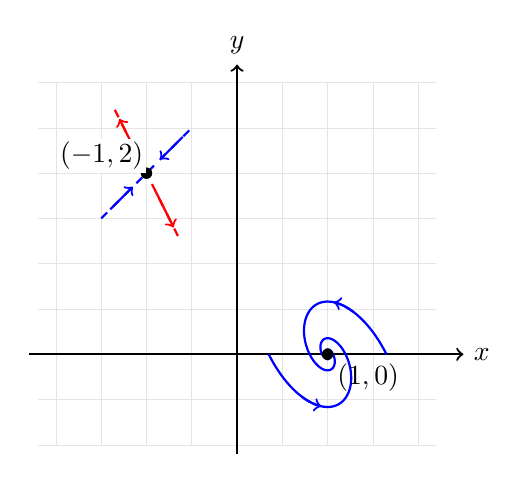
\begin{tikzpicture}[scale=1.15]
    \draw[step=0.5,very thin,gray!20]
        (-2.2,-1) grid (2.2,3);
    \draw[->,thick] (-2.3,0)--(2.5,0)
        node[right] {$x$};
    \draw[->,thick] (0,-1.1)--(0,3.2)
        node[above] {$y$};

    % Solutions of the linearized system near (1,0)
    \foreach \r in {-0.65,0.65}{
        \draw[blue,thick,domain=0:9,samples=300]
            plot
            ({1+\r*exp(-\x/2)*
                (cos(deg(sqrt(7)*\x/2))
                -sin(deg(sqrt(7)*\x/2))/sqrt(7))},
             {4*\r*exp(-\x/2)*
                sin(deg(sqrt(7)*\x/2))/sqrt(7)});

        \draw[blue,thick,->,domain=0.5:0.8,samples=25]
            plot
            ({1+\r*exp(-\x/2)*
                (cos(deg(sqrt(7)*\x/2))
                -sin(deg(sqrt(7)*\x/2))/sqrt(7))},
             {4*\r*exp(-\x/2)*
                sin(deg(sqrt(7)*\x/2))/sqrt(7)});
    }

    % Saddle: stable tangent direction
    \draw[blue,dashed,thick] (-1.5,1.5)--(-0.5,2.5);
    \draw[blue,thick,->] (-1.4,1.6)--(-1.15,1.85);
    \draw[blue,thick,->] (-0.6,2.4)--(-0.85,2.15);

    % Saddle: unstable tangent direction
    \draw[red,dashed,thick] (-1.35,2.7)--(-0.65,1.3);
    \draw[red,thick,->] (-1.1,2.2)--(-1.3,2.6);
    \draw[red,thick,->] (-0.9,1.8)--(-0.7,1.4);

    % Equilibria
    \fill (1,0) circle (1.8pt);
    \fill (-1,2) circle (1.8pt);
    \node[below right] at (1,0) {$(1,0)$};
    \node[above left,fill=white,inner sep=1pt]
        at (-1,2) {$(-1,2)$};
\end{tikzpicture}

\small
Local behavior predicted by the linearized systems.
Blue arrows point inward; red arrows point outward.
\end{center}

%-------------------------------------------------------------
\subsection{Extending the Sketch}

To guide the trajectories farther away, return
to the original equations:
\[
x'=1-x-y,\qquad y'=x^2-1.
\]
They give the following directions:
\[
\begin{aligned}
y<1-x&\implies x'>0,
&
y>1-x&\implies x'<0,\\
|x|>1&\implies y'>0,
&
|x|<1&\implies y'<0.
\end{aligned}
\]
The curves where one derivative vanishes are called
\textbf{nullclines}. Here they are
\[
y=1-x,\qquad x=-1,\qquad x=1.
\]

Use these signs together with the local behavior
to sketch trajectories. Do not extend the saddle
eigendirections as straight lines across the
entire plane.

\begin{figure}[H]
    \centering
    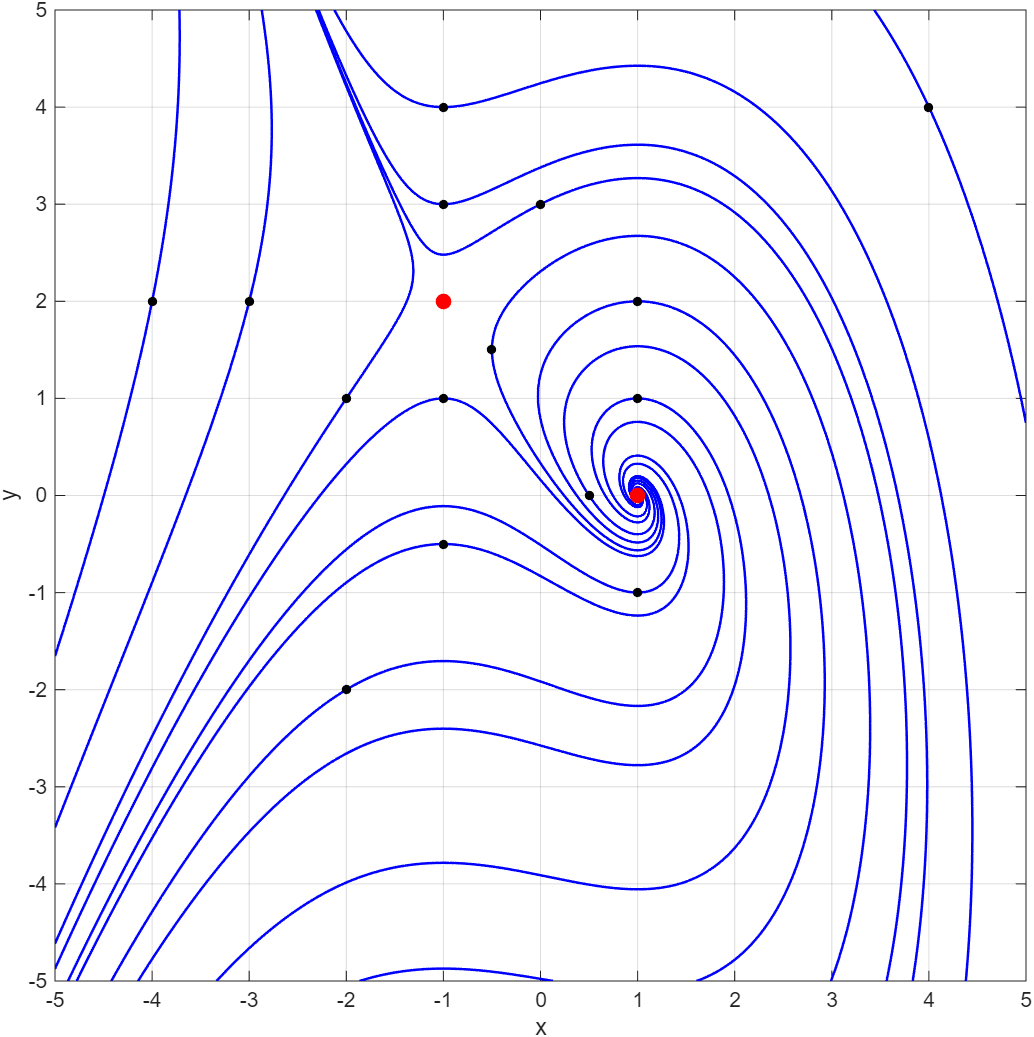
\includegraphics[width=0.7\linewidth]
        {figs/phase_saddle_spiral.png}
    \caption{A numerical phase portrait of the nonlinear
    system. The saddle trajectories curve away from
    their local tangent directions.}
\end{figure}

%%%%%%%%%%%%%%%%%%%%%%%%%%%%%%%%%%%%%%%%%%%%%%%%%%%%%%%%%%%%%%%%%%%%%%%%
\section{A Saddle and a Node}

\subsection{Finding and Classifying the Equilibria}

\begin{example}[2]{
Find and classify the equilibria, then sketch the
local behavior of
\[
\begin{dcases}
x'=x(y-4),\\
y'=y(x-1).
\end{dcases}
\]
}

\paragraph{Step 1. Find the equilibria.}
Set
\[
x(y-4)=0,\qquad y(x-1)=0.
\]
The first equation gives $x=0$ or $y=4$.

If $x=0$, the second equation becomes $-y=0$.
If $y=4$, the second equation becomes $4(x-1)=0$.

Therefore, the equilibria are
\[
\boxed{(0,0)\qquad\text{and}\qquad(1,4).}
\]

\paragraph{Step 2. Compute the Jacobian.}
The Jacobian is
\[
\boxed{
J(x,y)=
\begin{pmatrix}
y-4&x\\
y&x-1
\end{pmatrix}.
}
\]

\paragraph{Step 3. Classify $(0,0)$.}
At the origin,
\[
A_1=J(0,0)=
\begin{pmatrix}
-4&0\\
0&-1
\end{pmatrix}.
\]
For a diagonal matrix, the diagonal entries are
eigenvalues and the coordinate vectors are eigenvectors:
\[
\lambda_1=-4,\qquad
\mathbf{v}_1=\begin{pmatrix}1\\0\end{pmatrix},
\]
\[
\lambda_2=-1,\qquad
\mathbf{v}_2=\begin{pmatrix}0\\1\end{pmatrix}.
\]
Both eigenvalues are negative and distinct, so
\[
\boxed{(0,0)\text{ is an asymptotically stable node}.}
\]

The $x$-component decays faster than the $y$-component.
Generic nearby trajectories approach the origin
tangent to the slower direction, the $y$-axis.

\paragraph{Step 4. Classify $(1,4)$.}
At the second equilibrium,
\[
A_2=J(1,4)=
\begin{pmatrix}
0&1\\
4&0
\end{pmatrix}.
\]
The characteristic equation is
\[
\det(\lambda I-A_2)
=
\begin{vmatrix}
\lambda&-1\\
-4&\lambda
\end{vmatrix}
=\lambda^2-4=0.
\]
Thus,
\[
\lambda_u=2,\qquad \lambda_s=-2,
\]
and
\[
\boxed{(1,4)\text{ is a saddle}.}
\]

\paragraph{Step 5. Find the saddle eigendirections.}
For $\lambda_u=2$,
\[
A_2-2I=
\begin{pmatrix}
-2&1\\
4&-2
\end{pmatrix}
\implies
\mathbf{v}_u=\begin{pmatrix}1\\2\end{pmatrix}.
\]
For $\lambda_s=-2$,
\[
A_2+2I=
\begin{pmatrix}
2&1\\
4&2
\end{pmatrix}
\implies
\mathbf{v}_s=\begin{pmatrix}1\\-2\end{pmatrix}.
\]

The tangent lines through $(1,4)$ are
\[
\begin{aligned}
y-4&=2(x-1)
&&\text{unstable direction},\\
y-4&=-2(x-1)
&&\text{stable direction}.
\end{aligned}
\]
\end{example}

%-------------------------------------------------------------
\subsection{Sketching the Local Behavior}

At the origin, draw a stable node. The linearized
solutions are
\[
u(t)=c_1e^{-4t},
\qquad
v(t)=c_2e^{-t}.
\]
When $c_2\ne0$, eliminating $t$ gives
\[
u=Cv^4.
\]
Thus, these curves are tangent to the $v$-axis
at the origin; they are not parabolas.

At $(1,4)$, draw the stable and unstable saddle
directions found in Example 2.

\begin{center}
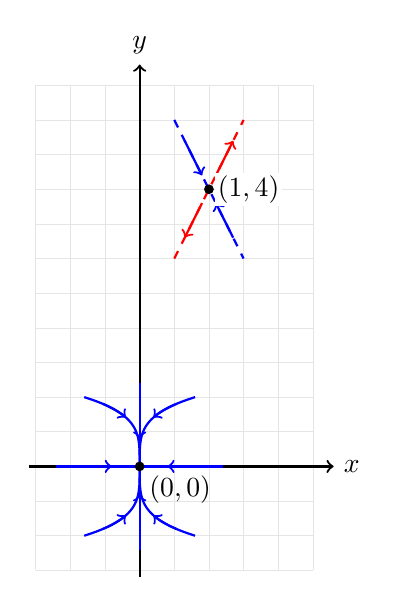
\begin{tikzpicture}[scale=0.88]
    \draw[step=0.5,very thin,gray!20]
        (-1.5,-1.5) grid (2.5,5.5);
    \draw[->,thick] (-1.6,0)--(2.8,0)
        node[right] {$x$};
    \draw[->,thick] (0,-1.6)--(0,5.8)
        node[above] {$y$};

    % Stable-node eigendirections
    \draw[blue,thick] (-1.2,0)--(1.2,0);
    \draw[blue,thick] (0,-1.2)--(0,1.2);
    \draw[blue,thick,->] (0.9,0)--(0.4,0);
    \draw[blue,thick,->] (-0.9,0)--(-0.4,0);
    \draw[blue,thick,->] (0,0.9)--(0,0.4);
    \draw[blue,thick,->] (0,-0.9)--(0,-0.4);

    % Representative linearized node trajectories
    \foreach \a/\b in {0.8/1,0.8/-1,-0.8/1,-0.8/-1}{
        \draw[blue,thick,domain=0:3,samples=100]
            plot
            ({\a*exp(-4*\x)},{\b*exp(-\x)});
        \draw[blue,thick,->,domain=0.1:0.35,samples=20]
            plot
            ({\a*exp(-4*\x)},{\b*exp(-\x)});
    }

    % Saddle at (1,4)
    \draw[red,dashed,thick] (0.5,3)--(1.5,5);
    \draw[blue,dashed,thick] (0.5,5)--(1.5,3);

    \draw[red,thick,->] (1.1,4.2)--(1.35,4.7);
    \draw[red,thick,->] (0.9,3.8)--(0.65,3.3);

    \draw[blue,thick,->] (0.65,4.7)--(0.9,4.2);
    \draw[blue,thick,->] (1.35,3.3)--(1.1,3.8);

    % Equilibria
    \fill (0,0) circle (2pt);
    \fill (1,4) circle (2pt);
    \node[below right] at (0,0) {$(0,0)$};
    \node[right,fill=white,inner sep=1pt]
        at (1.08,4) {$(1,4)$};
\end{tikzpicture}

\small
Local behavior predicted by the linearized systems.
Dashed lines show tangent directions at the saddle.
\end{center}

%-------------------------------------------------------------
\subsection{Using the Original Equations}

The original equations provide more information:
\[
x'=x(y-4),\qquad y'=y(x-1).
\]
In the first quadrant,
\[
\begin{aligned}
y<4&\implies x'<0,
&
y>4&\implies x'>0,\\
x<1&\implies y'<0,
&
x>1&\implies y'>0.
\end{aligned}
\]
Thus, the lines $x=1$ and $y=4$ separate regions
with different directions of motion.

The coordinate axes are exact invariant lines:
\[
y=0\implies y'=0,
\qquad
x=0\implies x'=0.
\]
The saddle eigendirections, however, generally
give only tangent lines to curved trajectories.

%-------------------------------------------------------------
\subsection{Local Information and Global Behavior}

Linearization gives local information. To construct
a larger phase portrait, we must also respect the
original vector field.

For these smooth systems:
\begin{itemize}
    \item Distinct trajectories cannot cross.
    \item Trajectories must follow the signs of
    $x'$ and $y'$.
    \item The local behavior must agree with the
    equilibrium classifications.
\end{itemize}

Non-intersection alone is not enough to determine
how trajectories connect. Use nullclines, the vector
field, or numerical solutions to resolve the global
behavior.

\begin{figure}[H]
    \centering
    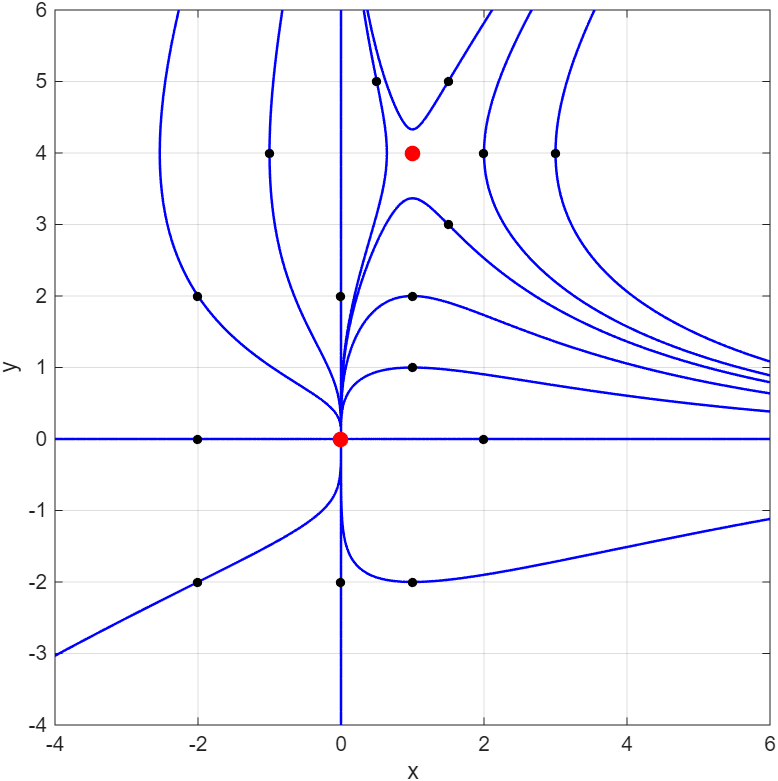
\includegraphics[width=0.7\linewidth]
        {figs/phase_saddle_node.png}
    \caption{A numerical phase portrait showing how
    the local behavior extends into the rest of
    the phase plane.}
\end{figure}

%%%%%%%%%%%%%%%%%%%%%%%%%%%%%%%%%%%%%%%%%%%%%%%%%%%%%%%%%%%%%%%%%%%%%%%%
\section{Population Models}

\subsection{Review of Logistic Growth}

Suppose $x(t)$ is the population of rabbits
in a forest. The \textbf{logistic model} is
\[
\boxed{
x'=r_1x\left(1-\frac{x}{K_1}\right),
\qquad r_1,K_1>0.
}
\]
Here,
\begin{itemize}
    \item $r_1$ is the intrinsic growth rate;
    \item $K_1$ is the carrying capacity.
\end{itemize}
For a positive initial population, the population
approaches $K_1$. It increases below carrying capacity
and decreases above it.

%-------------------------------------------------------------
\subsection{Noninteracting Species}

Suppose a second species has population $y(t)$
and does not interact with the rabbits. We can write
the two logistic equations as one system:
\[
\begin{dcases}
x'=r_1x\left(1-\dfrac{x}{K_1}\right),\\[4pt]
y'=r_2y\left(1-\dfrac{y}{K_2}\right).
\end{dcases}
\]
This system is \textbf{decoupled}: the equation for
$x$ depends only on $x$, and the equation for $y$
depends only on $y$.

Solving the system is the same as solving the
two equations separately.

%-------------------------------------------------------------
\subsection{Competing Species}

Now suppose $x$ and $y$ represent rabbits and deer
that compete for limited food or space. Their presence
reduces each other's growth rates.

A common model is
\[
\boxed{
\begin{dcases}
x'=r_1x\left(1-\dfrac{x}{K_1}\right)-\alpha xy,\\[4pt]
y'=r_2y\left(1-\dfrac{y}{K_2}\right)-\beta xy,
\end{dcases}
\qquad \alpha,\beta>0.
}
\]
The parameters $\alpha$ and $\beta$ describe
the strength of competition.

Both equations now depend on both populations,
so the system is \textbf{coupled}. The interaction
terms vanish if either species is absent and
become stronger when both populations are large.

%-------------------------------------------------------------
\subsection{Questions for Phase Plane Analysis}

A phase portrait can help us answer:
\begin{itemize}
    \item Does one species drive the other to extinction?
    \item Can both species coexist at a stable equilibrium?
    \item Does the outcome depend on the initial populations?
\end{itemize}

We investigate these questions by finding equilibria,
classifying them, and interpreting the trajectories
in the first quadrant.

\end{document}